\documentclass[aspectratio=169]{beamer} 
% 16:9 宽屏比例

\usepackage{../../Styles/mystyle-PPT}

\graphicspath{{./image/}}% 指定图片目录，后续可以直接使用图片文件名。

% --- 主题设置 ---
\usetheme{metropolis}
% \usetheme{Madrid} % 备选主题

% --- 颜色微调 ---
% 自定义颜色，接近PPT模板的青色和绿色
\definecolor{mycolor}{RGB}{0, 176, 183} % 青色
\definecolor{mycolor2}{RGB}{0, 191, 165} % 绿色
\usecolortheme[named=mycolor]{structure}


% --- 演示文稿基础信息 ---
\title{多元统计分析}
\subtitle{广义线性模型（GLM）数学理论与R语言实现}
\author{邹文杰}
\institute{哈尔滨商业大学}
\date{2026年4月}

\begin{document}

% 标题页
\begin{frame}
\titlepage
\end{frame}

% 目录页
\begin{frame}{目录 CONTENTS}
\begin{columns}[T]
\column{0.48\textwidth}
\begin{block}{01 一般线性模型回顾}
数学定义、基本假设与局限性
\end{block}
\begin{block}{02 GLM理论部分}
定义、指数族分布、核心定理、三要素解析
\end{block}
\begin{block}{03 GLM标准化建模流程}
数学步骤与实操流程
\end{block}
\column{0.48\textwidth}
\begin{block}{04 二项分布GLM实例}
逻辑回归·数学模型·R代码·结果解读
\end{block}
\begin{block}{05 泊松分布GLM实例}
计数回归·数学模型·R代码·结果解读
\end{block}
\begin{block}{06 课程总结}
理论梳理与方法归纳
\end{block}
\end{columns}
\end{frame}


\section{一般线性模型回顾}

\begin{frame}{一般线性模型：数学定义与假设}
\begin{block}{定义 一般线性模型}
设独立观测 $(Y_i, X_{i1},\cdots,X_{ip})$，模型形式为：
\[ Y_i = \beta_0+\beta_1X_{i1}+\cdots+\beta_pX_{ip}+\varepsilon_i \]
矩阵形式：$\boldsymbol{Y}=\boldsymbol{X\beta}+\boldsymbol{\varepsilon}$
\end{block}
\begin{block}{基本假设（Gauss-Markov）}
\begin{itemize}
\item 线性性：$\mathbb{E}(Y)=\boldsymbol{X\beta}$
\item 正态性：$\varepsilon_i\sim N(0,\sigma^2)$，即$Y\mid X\sim N(\mu,\sigma^2)$
\item 方差齐性：$\text{Var}(Y)=\sigma^2$（常数）
\item 独立性：$\varepsilon_i$相互独立
\end{itemize}
\end{block}
\begin{alertblock}{核心局限}
仅适用于\textbf{连续正态数据}，无法处理二分类/计数/偏态数据
\end{alertblock}
\end{frame}

\section{GLM理论部分}

\begin{frame}{指数族分布}
\begin{block}{定义 单参数指数族}
概率分布可表示为：
\[ f(y;\theta,\phi)=\exp\left\{\frac{y\theta-b(\theta)}{a(\phi)}+c(y,\phi)\right\} \]
\begin{itemize}
\item $\theta$：自然参数（决定均值）
\item $\phi$：离散参数（方差）
\item $b(\theta)$：累积量函数，满足$\mathbb{E}(Y)=b'(\theta),\ \text{Var}(Y)=a(\phi)b''(\theta)$
\end{itemize}
\end{block}
\begin{block}{常见指数族分布}
正态分布、二项分布、泊松分布、伽马分布均属于指数族
\end{block}
\end{frame}

\begin{frame}{广义线性模型（GLM）}
\begin{block}{定义 GLM的定义}
广义线性模型(GLM)是满足以下条件的统计模型：
\begin{enumerate}
\item 响应变量 $Y_1,\cdots,Y_n$ 独立且服从\textbf{指数族分布}

\item 存在严格单调可微函数 $g(\cdot)$，使得
\[ \boldsymbol{g(\mathbb{E}(Y)) = \eta = \boldsymbol{X\beta}}==\beta_0+\beta_1X_1+\cdots+\beta_pX_p \]
\end{enumerate}
其中：$\eta$为\textbf{线性预测子}，$\boldsymbol{\beta}$为待估参数向量，$g$为\textbf{连接函数}
\end{block}

\begin{block}{定义 典则连接}
若取$\eta = g(\mu) = \theta$,其中$\theta$为指数族分布中的自然参数,则称这样的$g$为\textbf{典则连接}
\end{block}
\begin{alertblock}{注}
连接函数的作用：将受限均值映射为全体实数

$g$的逆变换$g^{-1}(\eta)$一般要具有实际意义，例如：优势比、发生率。
\end{alertblock}
\end{frame}

\begin{frame}{GLM核心定理与性质}
\begin{block}{定理 OLS是GLM的特例}
当$Y\mid X\sim N(\mu,\sigma^2)$且连接函数$g(\mu)=\mu$时，GLM退化为一般线性模型
\end{block}
\begin{block}{定理 参数估计}
GLM参数采用\textbf{最大似然估计}（$\boldsymbol{MLE}$），通过迭代加权\textbf{最小二乘}（$\boldsymbol{IRLS}$）求解：
\[ \hat{\beta} \xrightarrow{d} N(\beta,(X^TWX)^{-1}) \]
具有一致性、渐近正态性
\end{block}
\begin{block}{关键性质}
GLM不要求方差齐性，方差$\text{Var}(Y)=V(\mu)$是均值的函数
\end{block}
\end{frame}


\section{GLM标准化建模流程}

\begin{frame}{GLM建模全流程（数学+实操）}
\begin{block}{$\mathbf{Step}$ 1 数据判定}
判定$Y$的分布类型。\,\,例如：连续→正态；二分类→二项；计数→泊松
\end{block}
\begin{block}{$\mathbf{Step}$ 2 模型设定}
选定分布+连接函数，构建$g(\mu)=\boldsymbol{X\beta}$，然后
确定GLM数学表达式
\end{block}
\begin{block}{$\mathbf{Step}$ 3 参数估计}
MLE+IRLS迭代求解$\hat{\beta}$。R语言glm()函数拟合
\end{block}
\begin{block}{$\mathbf{Step}$ 4 模型检验}
显著性检验、AIC、偏差检验。例如：P值<0.05为显著，AIC越小拟合越好
\end{block}
\begin{block}{$\mathbf{Step}$ 5 预测与解释}
逆变换$\mu=g^{-1}(\eta)$还原均值。\,\,例如：概率/计数预测，优势比/发生率比解读
\end{block}
\end{frame}


\section{二项分布GLM：逻辑回归}

\begin{frame}{二项GLM：数学模型与理论}
\begin{block}{定义 二项分布GLM}
\begin{itemize}
\item 随机部分：$Y_i\sim Binomial(1,\pi)$，$\pi=\mathbb{E}(Y)$
\item 连接函数：Logit典则连接
\[ g(\pi)=\text{logit}(\pi)=\ln\left(\frac{\pi}{1-\pi}\right) \]
\item 模型公式：$\ln\left(\frac{\pi}{1-\pi}\right)=\beta_0+\beta_1X_1+\cdots+\beta_pX_p$
\end{itemize}
\end{block}
\begin{block}{逆变换（预测）}
\[ \pi=\frac{\exp(\boldsymbol{X\beta})}{1+\exp(\boldsymbol{X\beta})}\in(0,1) \]
\end{block}
\end{frame}

\begin{frame}[fragile]{实例：研究生录取预测·R代码（tidyverse）}
\begin{block}{数据与建模}
\begin{lstlisting}[title=R代码]
# 加载tidyverse包
library(tidyverse)
# 读取UCLA录取数据
df <- read_csv("https://stats.idre.ucla.edu/stat/data/binary.csv")
# 数据预处理
df <- df %>% mutate(rank = factor(rank))
# 拟合二项GLM（逻辑回归）
model_bin <- glm(admit ~ gre + gpa + rank, 
data = df, family = binomial(link = "logit"))
# 模型结果
summary(model_bin)
\end{lstlisting}
\end{block}
\end{frame}

\begin{frame}{模型结果}
\begin{figure}[H]
\centering
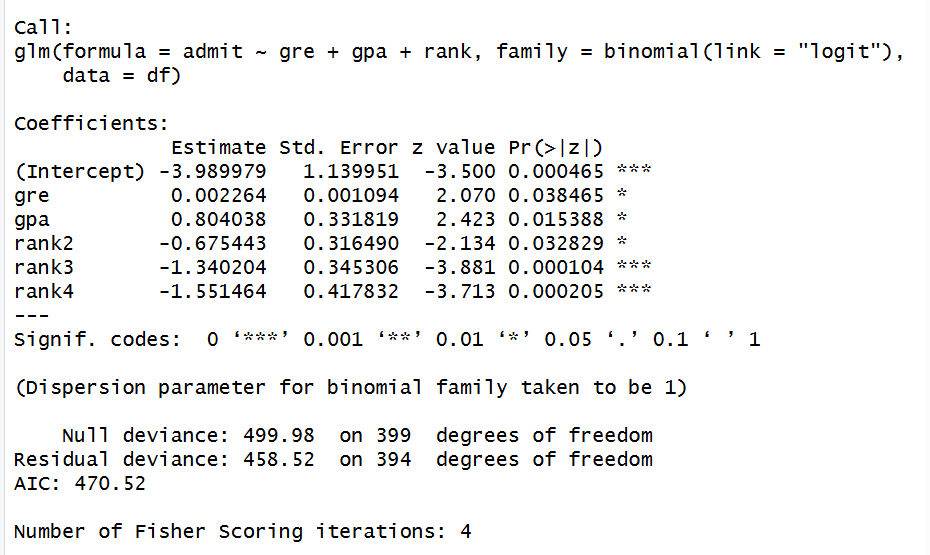
\includegraphics[scale=0.5]{R结果图1.png}
\caption{运行结果}
\label{figure:R结果图1}
\end{figure} 
\end{frame}

\begin{frame}{广义线性模型（逻辑回归）结果解释}
% 1. 系数显著性检验
\begin{block}{系数显著性检验}
截距、gre、gpa、rank2、rank3、rank4 均通过显著性检验（$P<0.05$），所有变量对录取结果均有显著影响
\end{block}

% 2. 最终模型公式（核心）
\begin{block}{最终回归模型（Logit形式）}
\begin{align*}
&\text{logit}(\hat{p}) = \ln\left( \frac{\hat{p}}{1-\hat{p}} \right) \\
&= -3.99 + 0.00226\ \text{gre} + 0.804\ \text{gpa} - 0.675\ \text{rank2} - 1.340\ \text{rank3} - 1.551\ \text{rank4}
\end{align*}
其中 $\hat{p}$ 表示考生被录取的概率。
\end{block}
\end{frame}

\begin{frame}{优势比(OR)解释}
\begin{block}{优势比(OR)解释}
优势比公式：\[ OR_j=\exp(\beta_j) \]
\begin{itemize}
\item $OR(\text{gre})=1.002$：GRE分数每增加1分，录取优势扩大为原来的1.002倍
\item $OR(\text{gpa})=2.23$：GPA每提升1分，录取优势扩大为原来的2.23倍
\item $OR(\text{rank2})=0.51$：rank2院校考生的录取优势为rank1的51\%
\item $OR(\text{rank3})=0.26$：rank3院校考生的录取优势为rank1的26\%
\item $OR(\text{rank4})=0.21$：rank4院校考生的录取优势为rank1的21\%
\end{itemize}
\end{block}
\end{frame}

\begin{frame}{模型拟合评价}
\begin{block}{模型拟合评价}
\begin{itemize}
\item 零偏差：$499.98\ (\text{df}=399)$，残差偏差：$458.52\ (\text{df}=394)$，偏差差 $\Delta\text{Deviance}=41.46$，自由度差$\text{df}=5$，整体显著（p<0.001）

\item 离散参数(残差偏差/零偏差)近似为1，无严重过离散问题，模型设定合理
\end{itemize}
\end{block}
\begin{alertblock}{注}
零偏差(Null deviance)：只有截距项的模型的偏差（完全不用自变量，只用样本均值预测）。

残差偏差(Residual deviance)：当前模型的偏差，代表模型无法解释的部分。

残差偏差<零偏差说明模型确实解释了一部分变量。
\end{alertblock}
\end{frame}

% ------------------------------
% 第五部分：泊松分布GLM（计数回归）
% ------------------------------
\section{泊松分布GLM：计数回归}

\begin{frame}{泊松GLM：数学模型与理论}
\begin{block}{定义 泊松分布GLM}
\begin{itemize}
\item 随机部分：$Y_i\sim Poisson(\lambda)$，$\lambda=\mathbb{E}(Y)>0$
\item 连接函数：对数典则连接
\[ g(\lambda)=\ln(\lambda) \]
\item 模型公式：$\ln(\lambda)=\beta_0+\beta_1X_1+\cdots+\beta_pX_p$
\end{itemize}
\end{block}
\begin{block}{逆变换}
\[ \lambda=\exp(\boldsymbol{X\beta})>0 \]
\end{block}
\end{frame}

\begin{frame}[fragile]{实例：织布断线次数分析·R代码（tidyverse）}
\begin{block}{数据与建模}
\begin{lstlisting}[title=R代码]
library(tidyverse)
# 加载R内置断线数据
data(warpbreaks)
# 拟合泊松GLM
model_pois <- glm(breaks ~ wool + tension, 
data = warpbreaks, family = poisson(link = "log"))
# 模型结果
summary(model_pois)
# 计算发生率比IRR
exp(coef(model_pois))# coef()提取回归系数
\end{lstlisting}
\end{block}
\end{frame}

\begin{frame}{模型结果}
\begin{figure}[H]
\centering
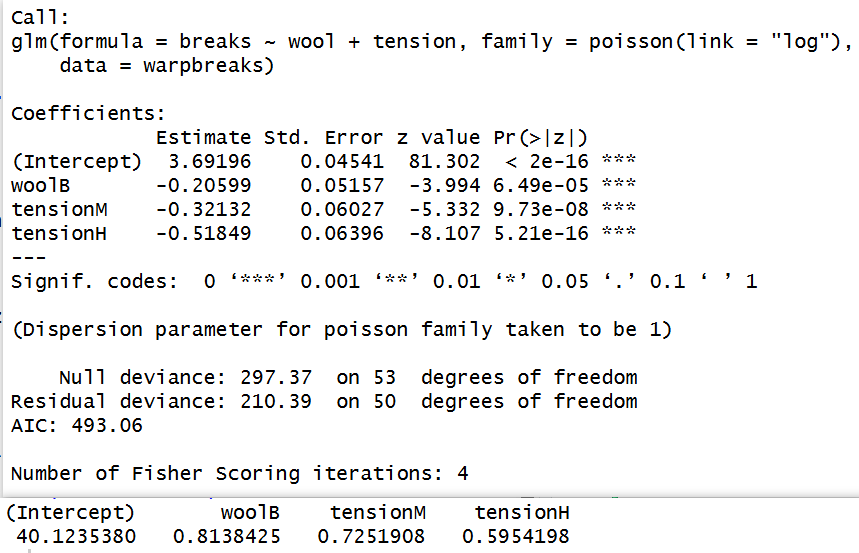
\includegraphics[scale=0.5]{R结果图2.png}
\caption{运行结果}
\label{figure:R结果图2}
\end{figure}
\end{frame}

\begin{frame}{结果解读与模型解释（泊松回归）}
% 1. 泊松回归模型公式（Log连接）
\begin{block}{泊松回归模型公式(Log连接)}
\[
\log(\lambda) = 3.692 - 0.206\ \text{woolB} - 0.321\ \text{tensionM} - 0.518\ \text{tensionH}
\]
其中 $\lambda = E(\text{breaks})$ 为断线次数的期望；
- $\text{wool}$ 以A类纱线为基准组，B类为哑变量；
- $\text{tension}$ 以低张力（L）为基准组，中/高张力为哑变量。
\end{block}

% 2. 系数显著性检验
\begin{block}{系数显著性检验}
所有变量系数的 $P$ 值均小于 $0.001$，表明：
$\text{wool}$ 类型与 $\text{tension}$ 张力水平对断线次数均有极显著影响。
\end{block}
\end{frame}

\begin{frame}
% 3. 发生率比（IRR）解释
\begin{block}{发生率比（IRR）解释}
泊松回归中，发生率比（Incidence Rate Ratio）公式为：
\[ IRR_j = \exp(\beta_j) \]
表示自变量每变化1单位，事件发生率变为原来的倍数：
\begin{itemize}
\item $\text{IRR}(\text{woolB})=0.81$：B类纱线的断线发生率为A类的81\%，即减少约19\%
\item $\text{IRR}(\text{tensionM})=0.73$：中张力下断线发生率为低张力的73\%，即减少约27\%
\item $\text{IRR}(\text{tensionH})=0.60$：高张力下断线发生率为低张力的60\%，即减少约40\%
\end{itemize}
\end{block}

% 4. 模型拟合评价
\begin{block}{模型拟合评价}
\begin{itemize}
\item 零偏差：$297.37\ (\text{df}=53)$，残差偏差：$210.39\ (\text{df}=50)$，偏差差 $\Delta\text{Deviance}=86.98$，自由度差$\text{df}=3$，整体显著（$p<0.001$）

\item 离散参数(残差偏差/零偏差)近似为1，无严重过离散问题，模型设定合理
\end{itemize}
\end{block}
\end{frame}


\section{课程总结}

\begin{frame}{总结与理论梳理}
\begin{columns}[T]
\column{0.48\textwidth}
\begin{block}{GLM核心理论}
\begin{itemize}
\item 基于指数族分布，突破正态假设
\item 连接函数完成均值→线性预测子映射
\item OLS是GLM的特例
\item MLE估计，IRLS求解
\end{itemize}
\end{block}
\column{0.48\textwidth}
\begin{block}{两大经典模型}
\begin{itemize}
\item 二分类数据：二项GLM+logit连接→逻辑回归
\item 计数数据：泊松GLM+log连接→计数回归
\item 统一用glm()实现
\end{itemize}
\end{block}
\end{columns}
\begin{block}{核心结论}
GLM是线性模型的公理级拓展，是处理非正态数据的标准统计方法
\end{block}
\end{frame}

% 结束页
\begin{frame}
\centering
\Huge \textcolor{mycolor}{感谢观看} \\
\vspace{0.3cm}
\Large THANKS FOR WATCHING
\end{frame}

\end{document}